% !TeX root = ../Baocao.tex
\section{Thực nghiệm và đánh giá kết quả}

Chương này xây dựng quy trình thực nghiệm để đánh giá toàn bộ chuỗi xử lý từ camera IMX500, bộ phát hiện ArUco, bộ điều khiển hạ cánh, ROS~2--PX4 bridge đến đáp ứng thực tế của UAV. Các thử nghiệm được triển khai theo mức độ rủi ro tăng dần: kiểm tra tĩnh trên mặt đất, kiểm tra truyền thông khi tháo cánh quạt, kiểm tra bộ điều khiển bằng thao tác thủ công, bay quan sát trong chế độ Position và cuối cùng mới thử nghiệm hạ cánh vòng kín. Trình tự này giúp tách biệt lỗi thị giác, lỗi truyền thông và lỗi điều khiển trước khi vận hành đầy đủ hệ thống.

\subsection{Mục tiêu và điều kiện thực nghiệm}

Mục tiêu thực nghiệm là kiểm chứng ba nhóm chức năng. Thứ nhất, camera và ArUco detector phải nhận đúng marker mục tiêu, cung cấp pose ổn định trong miền khoảng cách và góc quan sát dự kiến. Thứ hai, cầu nối uXRCE-DDS phải trao đổi dữ liệu hai chiều ổn định giữa Raspberry Pi~5 và NxtPx4V2, đồng thời các điều kiện an toàn phải ngăn việc chuyển sang Offboard khi trạng thái PX4 không hợp lệ. Thứ ba, bộ điều khiển phải đưa UAV hội tụ về tâm marker, chuyển pha đúng điều kiện và hoàn thành hạ cánh với sai số nằm trong giới hạn cho phép.

Các điều kiện chung cần được giữ cố định hoặc ghi lại trong từng lần thử được tổng hợp trong Bảng~\ref{tab:experimental_conditions}. Việc ghi nhận đầy đủ các điều kiện này giúp so sánh kết quả giữa các phiên thử và truy tìm nguyên nhân khi hệ thống hoạt động không ổn định.

\begin{table}[H]
    \centering
    \small
    \caption{Điều kiện chung của các thử nghiệm}
    \label{tab:experimental_conditions}
    \begin{tabularx}{\textwidth}{>{\raggedright\arraybackslash}p{0.30\textwidth} X}
        \toprule
        \textbf{Thông số} & \textbf{Cấu hình hoặc nội dung cần ghi nhận} \\
        \midrule
        Không gian thử nghiệm & Trong nhà, khu vực bằng phẳng, không có người và vật cản trong vùng bay. \\
        Marker mục tiêu & ArUco ID~0, từ điển \texttt{DICT\_5X5\_100}, kích thước cạnh $0{,}16$~m. \\
        Camera & IMX500 hướng xuống, độ phân giải $640\times480$; mép trên ảnh hướng về mũi UAV. \\
        Máy tính nhúng & Raspberry Pi~5 chạy Raspberry Pi OS và ROS~2 Humble trong Docker. \\
        Bộ điều khiển bay & NxtPx4V2, PX4 v1.17; kết nối UART ở $921600$ baud. \\
        Độ cao bắt đầu & Ghi lại theo từng lần thử; giá trị đề xuất cho thử nghiệm hoàn chỉnh là khoảng $1{,}5$~m. \\
        Điều kiện ánh sáng & Ghi mức độ chiếu sáng, hướng nguồn sáng, bóng đổ và hiện tượng phản xạ trên marker. \\
        Thông số điều khiển & Lưu phiên bản file cấu hình, hệ số PID, giới hạn vận tốc và ngưỡng chuyển pha. \\
        Dữ liệu ghi lại & Rosbag, log PX4, trạng thái ArUco, trạng thái landing, dữ liệu tài nguyên và video thử nghiệm. \\
        An toàn & Có vùng bay cách ly, công tắc dừng khẩn cấp và người điều khiển sẵn sàng chuyển về Position mode. \\
        \bottomrule
    \end{tabularx}
\end{table}

Trước mỗi lần bay, cần kiểm tra cánh quạt, chiều quay động cơ, pin, liên kết điều khiển từ xa, trạng thái estimator, local position, failsafe và khả năng chuyển về Position mode. Các thử nghiệm giao tiếp hoặc Offboard trên bàn phải tháo toàn bộ cánh quạt và giữ FC ở trạng thái disarmed.

\subsection{Các tiêu chí đánh giá}

Các tiêu chí đánh giá được chia thành bốn nhóm gồm hiệu năng thị giác, độ chính xác pose, chất lượng hạ cánh và độ ổn định của máy tính đồng hành. Bảng~\ref{tab:evaluation_metrics} định nghĩa các đại lượng chính cần thu thập.

\begin{table}[H]
    \centering
    \small
    \caption{Các tiêu chí đánh giá hệ thống}
    \label{tab:evaluation_metrics}
    \begin{tabularx}{\textwidth}{>{\raggedright\arraybackslash}p{0.27\textwidth} >{\raggedright\arraybackslash}p{0.18\textwidth} X}
        \toprule
        \textbf{Đại lượng} & \textbf{Đơn vị} & \textbf{Phương pháp xác định} \\
        \midrule
        Tần số camera và detector & frame/s & Đếm số frame hoặc số pose hợp lệ trong một khoảng thời gian xác định. \\
        Độ trễ detector & ms & Đọc trường \texttt{latency\_ms} trên \texttt{/uav/aruco/status}. \\
        Khoảng cách phát hiện tối đa & m & Tăng dần khoảng cách cho đến khi marker không còn được nhận ổn định. \\
        Sai số pose $X,Y,Z$ & m & So sánh \texttt{tvec} với vị trí marker được đo bằng thước hoặc giá thử. \\
        Độ dao động pose & m & Tính độ lệch chuẩn của từng thành phần pose khi camera và marker đứng yên. \\
        Sai số hạ cánh cuối & m & Đo khoảng cách giữa tâm marker và điểm tiếp xúc của cơ cấu gắp sau khi hạ cánh. \\
        Thời gian hạ cánh & s & Tính từ lúc bắt đầu quy trình Landing đến khi PX4 báo landed. \\
        Số lần mất marker & lần & Đếm các khoảng mà \texttt{target\_visible=false} trong pha tiếp cận bằng thị giác. \\
        Tỷ lệ thành công & \% & Tỷ số giữa số lần hạ cánh đạt yêu cầu và tổng số lần thử. \\
        CPU, RAM và nhiệt độ Pi & \%, MB, $^\circ$C & Ghi định kỳ trong toàn bộ phiên thử nghiệm. \\
        Điện áp và cảnh báo nguồn & V & Ghi điện áp thấp nhất và trạng thái undervoltage/throttling của Raspberry Pi. \\
        \bottomrule
    \end{tabularx}
\end{table}

Đối với các đại lượng thay đổi theo thời gian như pose, vận tốc điều khiển và nhiệt độ, cần lưu toàn bộ chuỗi mẫu thay vì chỉ ghi một giá trị tức thời. Kết quả nên được biểu diễn bằng giá trị trung bình, độ lệch chuẩn, giá trị cực đại và đồ thị theo thời gian.

\subsection{Thử nghiệm độ ổn định của hệ thống cấp nguồn}

Trước khi thực hiện các thử nghiệm liên quan đến camera và điều khiển, hệ thống cấp nguồn cho máy tính đồng hành được kiểm tra riêng để loại trừ nguyên nhân gây mất ổn định do sụt áp. Raspberry Pi~5 được cấp nguồn theo đúng cấu hình dự kiến khi bay: pin LiPo đi qua bộ hạ áp XL4015, sau đó đưa vào các chân $5$~V và GND trên GPIO. Trong thử nghiệm này, toàn bộ cánh quạt được tháo, bộ phát hiện ArUco chạy với camera IMX500 ở độ phân giải $640\times480$ và tốc độ $15$~frame/s, đồng thời Micro XRCE-DDS Agent được giữ hoạt động. Bộ điều khiển hạ cánh và yêu cầu Offboard không được kích hoạt.

Trong thời gian $10$ phút, dữ liệu được lấy mẫu mỗi giây, gồm điện áp rail $5$~V tại PMIC, nhiệt độ CPU, nhiệt độ PMIC, mức sử dụng CPU, tần số CPU, dung lượng bộ nhớ sử dụng và cờ throttling. Kết quả của phiên thử được tổng hợp trong Bảng~\ref{tab:power_stability_result}.

\begin{table}[H]
    \centering
    \small
    \caption{Kết quả thử nghiệm độ ổn định nguồn Raspberry Pi~5}
    \label{tab:power_stability_result}
    \begin{tabularx}{\textwidth}{>{\raggedright\arraybackslash}p{0.46\textwidth} X}
        \toprule
        \textbf{Đại lượng} & \textbf{Kết quả} \\
        \midrule
        Số mẫu và chu kỳ lấy mẫu & $600$ mẫu, $1$~s/mẫu \\
        Điện áp EXT5V\_V trung bình & $5{,}0002$~V \\
        Điện áp EXT5V\_V nhỏ nhất--lớn nhất & $4{,}8923$--$5{,}0384$~V \\
        Nhiệt độ CPU trung bình--cực đại & $70{,}4$--$74{,}1$~$^\circ$C \\
        Nhiệt độ PMIC trung bình--cực đại & $65{,}2$--$66{,}5$~$^\circ$C \\
        Mức sử dụng CPU trung bình--cực đại & $27{,}9$--$30{,}1$~\% \\
        Số mẫu có cờ throttling khác không & $0/600$ \\
        Số sự kiện undervoltage mới trong kernel & $0$ \\
        Dòng điện đầu vào & Chưa có sensor để đo \\
        \bottomrule
    \end{tabularx}
\end{table}

Các Hình~\ref{fig:power_cpu_usage}--\ref{fig:power_voltage} cho thấy điện áp cấp được duy trì xấp xỉ $5$~V trong suốt phiên thử, trong khi nhiệt độ CPU tăng rồi tiến tới vùng ổn định quanh $70$--$74~^\circ$C. Không xuất hiện sự kiện undervoltage mới và không có mẫu nào mang cờ throttling. Kết quả này chứng minh đường cấp nguồn GPIO hoạt động ổn định trong điều kiện tải tĩnh gồm camera, ArUco và Docker. Tuy nhiên, dòng điện đầu vào chưa được đo, đồng thời chưa đánh giá các quá độ do động cơ, servo hoặc điện áp LiPo thấp; vì vậy kết quả chỉ được xem là khảo sát tính khả thi ban đầu và chưa thay thế kiểm tra nguồn trong điều kiện bay.

\begin{figure}[H]
    \centering
    \includegraphics[width=0.95\textwidth]{power_test/04-power-cpu-usage.png}
    \caption{Mức sử dụng CPU của Raspberry Pi~5 khi chạy camera IMX500 và ArUco trong 10 phút.}
    \label{fig:power_cpu_usage}
\end{figure}

\begin{figure}[H]
    \centering
    \includegraphics[width=0.95\textwidth]{power_test/04-power-temperature.png}
    \caption{Nhiệt độ CPU và PMIC của Raspberry Pi~5 trong thời gian thử nghiệm.}
    \label{fig:power_temperature}
\end{figure}

\begin{figure}[H]
    \centering
    \includegraphics[width=0.95\textwidth]{power_test/04-power-voltage.png}
    \caption{Điện áp rail 5~V cấp cho Raspberry Pi~5 trong thời gian thử nghiệm.}
    \label{fig:power_voltage}
\end{figure}

\subsection{Thử nghiệm camera và ArUco tĩnh}

Các thử nghiệm tĩnh được thực hiện trước khi kết nối thuật toán với PX4. Camera được cố định, marker được đặt tại các vị trí đã đo trước, còn bộ điều khiển PID và PX4 bridge giữ ở trạng thái vô hiệu. Mỗi cấu hình nên được ghi tối thiểu từ $100$ đến $200$ mẫu pose để đánh giá độ ổn định.

\subsubsection{Ảnh hưởng của khoảng cách}

Marker ID~0 được đặt gần tâm ảnh tại ba khoảng cách danh định $0{,}50$, $0{,}80$ và $1{,}00$~m.
\begin{figure}[H]
    \centering
    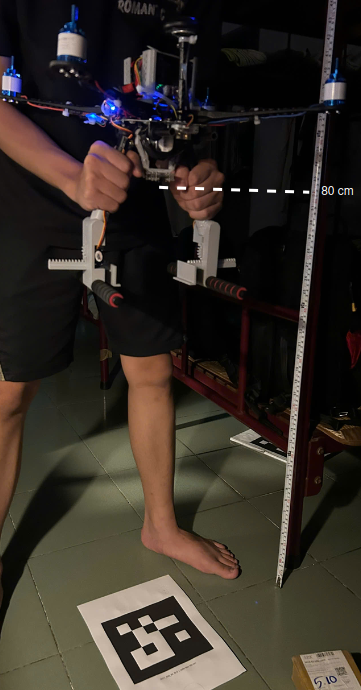
\includegraphics[width=0.3\textwidth]{images/04-space_test.png}
    \caption{Bố trí thực nghiệm ước lượng độ cao.}
    \label{fig:space-test}
\end{figure}

Mỗi phiên ghi rosbag trong khoảng 30~s, sau đó các mẫu trên các topic \texttt{/uav/aruco/ids}, \texttt{/uav/aruco/tvecs} và \texttt{/uav/aruco/status} được dùng để tính trung bình, độ lệch chuẩn, tần số phát hiện và độ trễ. Bảng~\ref{tab:aruco_distance_test} trình bày số liệu thu được.

\begin{table}[H]
    \centering
    \caption{Kết quả thử nghiệm ArUco theo khoảng cách}
    \label{tab:aruco_distance_test}
    \setlength{\tabcolsep}{5pt}
    \renewcommand{\arraystretch}{1.25}
    \begin{tabular}{c c c c c c c}
        \toprule
        \textbf{\shortstack{$Z$ đặt\\(m)}} &
        \textbf{\shortstack{ID~0 /\\phát hiện}} &
        \textbf{\shortstack{$\bar{x}$\\(m)}} &
        \textbf{\shortstack{$\bar{y}$\\(m)}} &
        \textbf{\shortstack{$\bar{z}\pm\sigma_z$\\(m)}} &
        \textbf{\shortstack{Độ trễ\\(ms)}} &
        \textbf{\shortstack{Tần số\\(Hz)}} \\
        \midrule
        $0{,}50$ & $182/188$ ($96{,}8\%$) & $-0{,}0055$ & $-0{,}0081$ & $0{,}5493\pm0{,}0389$ & $155{,}7$ & $6{,}19$ \\
        $0{,}80$ & $194/194$ ($100\%$) & $0{,}0066$ & $0{,}0458$ & $0{,}7845\pm0{,}0038$ & $147{,}3$ & $6{,}76$ \\
        $1{,}00$ & $151/165$ ($91{,}5\%$) & $0{,}0402$ & $-0{,}0073$ & $1{,}0039\pm0{,}0035$ & $177{,}5$ & $5{,}13$ \\
        \bottomrule
    \end{tabular}
\end{table}

\begin{figure}[H]
    \centering
    \includegraphics[width=1\textwidth]{aruco_static/04-aruco-z-distance-tests.png}
    \caption{Biến thiên thành phần $z$ của \texttt{tvec} trong ba phiên thử ArUco tĩnh. Đường gạch đỏ là khoảng cách danh định.}
    \label{fig:aruco_distance_z}
\end{figure}

Đồ thị trong Hình~\ref{fig:aruco_distance_z} thể hiện trực tiếp khoảng cách $z$ được bộ giải PnP ước lượng trong phép thử tĩnh. Tại $0{,}80$~m và $1{,}00$~m, giá trị ước lượng nằm gần khoảng cách danh định với độ lệch chuẩn lần lượt là $3{,}8$ và $3{,}5$~mm. Ở phiên danh định $0{,}50$~m, marker ban đầu được đặt lệch xa khoảng $10$~cm; các mẫu đầu vì vậy nằm quanh $0{,}60$--$0{,}65$~m. Khi marker được kéo xuống gần mốc thử, giá trị $z$ giảm liên tục và ổn định quanh $0{,}53$--$0{,}55$~m. Như vậy, đồ thị phản ánh đúng sự thay đổi khoảng cách thực tế trong lúc bố trí marker; giá trị trung bình toàn phiên tăng lên $0{,}549$~m và độ lệch chuẩn đạt $38{,}9$~mm chủ yếu do đoạn quá độ ban đầu, không phải do sai số ngẫu nhiên kéo dài của detector.

Tỷ lệ nhận đúng ID~0 đạt $100\%$ ở $0{,}80$~m, giảm còn $96{,}8\%$ ở $0{,}50$~m và $91{,}5\%$ ở $1{,}00$~m. Ở khoảng cách $1{,}00$~m, số lần mất marker tăng nhẹ và tần số xuất bản tvec giảm còn $5{,}13$~Hz; đây là vùng cần tiếp tục kiểm tra khi bay. Độ lệch trung bình theo phương ngang vẫn nhỏ, ngoại trừ thành phần $y=0{,}0458$~m tại $0{,}80$~m và $x=0{,}0402$~m tại $1{,}00$~m, cho thấy việc đặt marker bằng tay chưa hoàn toàn trùng tâm camera. Độ trễ đo được trong khoảng $147{,}3$--$177{,}5$~ms là thông số cần ghi nhận khi thiết kế và hiệu chỉnh PID ở các thí nghiệm sau.

Khoảng cách phát hiện ổn định không nên được xác định từ một frame đơn lẻ. Với ba phiên đo này, detector nhận dạng đáng tin cậy trong khoảng $0{,}50$--$1{,}00$~m, nhưng bộ điều khiển vẫn nên dùng điều kiện khóa nhiều frame liên tiếp và bộ lọc pose để loại bỏ quá độ hoặc các khoảng mất marker ngắn.

\subsubsection{Ảnh hưởng của vị trí marker trong ảnh}

Marker được đặt tại ba cấu hình đã ghi rosbag: chính giữa (center), bên phải (right) và một phiên di chuyển đa hướng (multidirectional3). Mục tiêu của phép thử là kiểm chứng đồng thời dấu của pose trong hệ camera quang học và chiều lệnh vận tốc sau khi bộ điều khiển biến đổi sang hệ body-FLU. Với camera quang học hiện tại, $x>0$ biểu thị marker nằm về phía phải ảnh, $y<0$ biểu thị marker nằm về phía trước ảnh; trong hệ body-FLU, $v_x>0$ là chuyển động về phía trước và $v_y<0$ là chuyển động sang phải. Vì vậy, khi dấu của sai số $x,y$ thay đổi, hai thành phần ngang của \texttt{cmd\_vel} cũng phải đổi chiều để giảm sai số tương ứng.

Các phiên center và right được ghi ở độ cao danh định $1{,}1208$~m. Phiên multidirectional3 kéo dài $42{,}25$~s, trong đó UAV/marker được xê dịch tuần tự qua nhiều hướng ở độ cao đo được khoảng $1{,}29$~m để quan sát đáp ứng theo thời gian; do đó đây là phép thử động trên mặt đất, không phải phép đo tĩnh thuần túy. Kết quả pose được tổng hợp trong Bảng~\ref{tab:marker_position_pose_result}.

\begin{table}[H]
    \centering
    \small
    \caption{Kết quả pose ArUco theo vị trí marker trong ảnh}
    \label{tab:marker_position_pose_result}
    \setlength{\tabcolsep}{4pt}
    \begin{tabular}{l c c c c c}
        \toprule
        \textbf{Vị trí} & \textbf{Số mẫu} & \textbf{$\bar{x}\pm\sigma_x$ (m)} & \textbf{$\bar{y}\pm\sigma_y$ (m)} & \textbf{$\bar{z}\pm\sigma_z$ (m)} & \textbf{Độ trễ (ms)} \\
        \midrule
        Center & $154$ & $-0{,}0075\pm0{,}0003$ & $0{,}0100\pm0{,}0018$ & $1{,}1228\pm0{,}0023$ & $175{,}6$ \\
        Right & $217$ & $0{,}1643\pm0{,}0006$ & $0{,}0550\pm0{,}0011$ & $1{,}1189\pm0{,}0047$ & $178{,}1$ \\
        Multidirectional3 & $233$ & $0{,}0133\pm0{,}1379$ & $0{,}0564\pm0{,}1341$ & $1{,}2941\pm0{,}0304$ & $180{,}3$ \\
        \bottomrule
    \end{tabular}
\end{table}

Mỗi cấu hình được biểu diễn bằng một đồ thị gồm bốn đường: pose $x,y$ và lệnh vận tốc body-FLU $v_x,v_y$. Hai đại lượng dùng hai trục tung riêng vì khác đơn vị; đường liền biểu diễn pose (m), đường nét đứt biểu diễn vận tốc (m/s). Rosbag center được ghi trước khi bổ sung topic \texttt{/aruco\_land/cmd\_vel}, vì vậy phần lệnh trong đồ thị center được đánh dấu là chưa có dữ liệu thay vì suy diễn từ pose.

\begin{figure}[H]
    \centering
    \includegraphics[width=0.98\textwidth]{aruco_static/04-aruco-center-pose-cmdvel-xy.png}
    \caption{Pose $x,y$ và lệnh \texttt{cmd\_vel.x,y} của cấu hình center.}
    \label{fig:aruco_center_pose_cmdvel_xy}
\end{figure}

\begin{figure}[H]
    \centering
    \includegraphics[width=0.98\textwidth]{aruco_static/04-aruco-right-pose-cmdvel-xy.png}
    \caption{Pose $x,y$ và lệnh \texttt{cmd\_vel.x,y} của cấu hình right.}
    \label{fig:aruco_right_pose_cmdvel_xy}
\end{figure}

\begin{figure}[H]
    \centering
    \includegraphics[width=0.98\textwidth]{aruco_static/04-aruco-multidirectional3-pose-cmdvel-xy.png}
    \caption{Pose $x,y$ và lệnh \texttt{cmd\_vel.x,y} khi di chuyển marker theo nhiều hướng.}
    \label{fig:aruco_multidirectional_pose_cmdvel_xy}
\end{figure}

Các giá trị trung bình của hai thành phần lệnh ngang được trình bày trong Bảng~\ref{tab:marker_position_cmd_result}. Ở cấu hình right, pose có $x>0$ và $y>0$ trong hệ camera, tương ứng bộ điều khiển phát $v_x=-0{,}0459$ và $v_y=-0{,}0942$~m/s để đưa UAV lùi lại và dịch sang phải. Ở phiên multidirectional3, các giá trị trung bình trên toàn phiên là $v_x=-0{,}0447$ và $v_y=-0{,}0090$~m/s. Hai giá trị này chỉ mang tính mô tả toàn phiên vì marker được đưa qua nhiều góc phần tư; dấu và biên độ tức thời cần được đọc trên Hình~\ref{fig:aruco_multidirectional_pose_cmdvel_xy}. Khi $x,y$ đổi dấu, các đường nét đứt cũng đảo chiều hoặc tiến về không, cho thấy bộ điều khiển đang phản hồi theo sai số ngang thay vì giữ một lệnh cố định.

\begin{table}[H]
    \centering
    \small
    \caption{Giá trị trung bình của lệnh vận tốc theo vị trí marker}
    \label{tab:marker_position_cmd_result}
    \setlength{\tabcolsep}{5pt}
    \begin{tabular}{l c c c}
        \toprule
        \textbf{Vị trí} & \textbf{Số mẫu} & \textbf{$\bar{v}_x$ (m/s)} & \textbf{$\bar{v}_y$ (m/s)} \\
        \midrule
        Center & -- & \multicolumn{2}{c}{Chưa ghi topic \texttt{/aruco\_land/cmd\_vel}} \\
        Right & $775$ & $-0{,}0459$ & $-0{,}0942$ \\
        Multidirectional3 & $846$ & $-0{,}0447$ & $-0{,}0090$ \\
        \bottomrule
    \end{tabular}
\end{table}

Trong phiên multidirectional3, $x$ thay đổi từ $-0{,}242$ đến $0{,}272$~m và $y$ từ $-0{,}161$ đến $0{,}342$~m; marker vẫn được nhận ở cả $233/233$ mẫu pose và bộ điều khiển duy trì trạng thái \texttt{visual\_approach}, không phát sinh \texttt{abort}. Do đó, đồ thị cho thấy rõ miền biến thiên pose và sự thay đổi tương ứng của lệnh ngang trong bài thử bench; kết quả này chưa phải là đánh giá hạ cánh khi UAV đang bay.

\subsubsection{Ảnh hưởng của góc nghiêng}

Marker được nghiêng lần lượt $0^\circ$, $15^\circ$, $30^\circ$ và $45^\circ$ trong khi giữ gần như không đổi khoảng cách đến camera. Tại mỗi góc, cần ghi tỷ lệ nhận đúng ID, độ trễ và độ dao động của các thành phần pose. Kết quả cho phép xác định miền góc quan sát mà detector còn đủ tin cậy để sử dụng cho visual servoing.

\begin{table}[H]
    \centering
    \small
    \caption{Mẫu kết quả thử nghiệm theo góc nghiêng marker}
    \label{tab:marker_tilt_test}
    \begin{tabularx}{\textwidth}{c c c c X}
        \toprule
        \textbf{Góc nghiêng} & \textbf{Tỷ lệ phát hiện} & \textbf{Độ trễ} & \textbf{Độ lệch chuẩn pose} & \textbf{Nhận xét} \\
        \midrule
        $0^\circ$ & -- & -- & -- & -- \\
        $15^\circ$ & -- & -- & -- & -- \\
        $30^\circ$ & -- & -- & -- & -- \\
        $45^\circ$ & -- & -- & -- & -- \\
        \bottomrule
    \end{tabularx}
\end{table}

\subsubsection{Ảnh hưởng của điều kiện ánh sáng}

Bốn trường hợp được khảo sát gồm ánh sáng đầy đủ, ánh sáng yếu, marker xuất hiện bóng đổ và marker bị che một phần. Camera giữ nguyên cấu hình để kết quả phản ánh trực tiếp độ bền vững của detector. Ngoài tỷ lệ phát hiện và độ trễ, cần ghi nhận hiện tượng nhòe ảnh hoặc thay đổi thời gian phơi sáng nếu có.

\begin{table}[H]
    \centering
    \small
    \caption{Mẫu kết quả thử nghiệm theo điều kiện quan sát}
    \label{tab:lighting_test}
    \begin{tabularx}{\textwidth}{>{\raggedright\arraybackslash}p{0.25\textwidth} c c X}
        \toprule
        \textbf{Điều kiện} & \textbf{Tỷ lệ phát hiện} & \textbf{Độ trễ} & \textbf{Nhận xét chất lượng pose} \\
        \midrule
        Ánh sáng đầy đủ & -- & -- & -- \\
        Ánh sáng yếu & -- & -- & -- \\
        Có bóng đổ & -- & -- & -- \\
        Marker bị che một phần & -- & -- & -- \\
        \bottomrule
    \end{tabularx}
\end{table}

\subsection{Thử nghiệm kết nối ROS 2--PX4}

Nhóm thử nghiệm này xác nhận đường truyền dữ liệu và các khóa an toàn trước khi điều khiển động cơ. Toàn bộ cánh quạt phải được tháo, FC giữ disarmed và các setpoint ban đầu bằng không.

\subsubsection{Kiểm tra uXRCE-DDS}

Micro XRCE-DDS Agent được khởi động với cổng \texttt{/dev/ttyAMA0} và baudrate $921600$. Thử nghiệm đạt yêu cầu khi agent nhận client từ PX4, các topic \texttt{/fmu/in/*} và \texttt{/fmu/out/*} xuất hiện, đồng thời đọc được dữ liệu thay đổi hợp lý từ attitude, vehicle status và local position. Cần kiểm tra liên tục trong vài phút để phát hiện mất kết nối ngắt quãng hoặc lỗi tăng dần theo thời gian.

\subsubsection{Kiểm tra Offboard khi tháo cánh quạt}

Sau khi xác nhận local position và attitude hợp lệ, bridge được enable trong khi setpoint vận tốc bằng không. Hệ thống phát heartbeat và setpoint đủ lâu trước khi gửi yêu cầu Offboard. Kết quả cần được xác nhận đồng thời bằng \texttt{VehicleCommandAck}, \texttt{VehicleStatus} và log của bridge. Tiếp theo, chủ động dừng luồng setpoint để kiểm tra PX4 rời Offboard hoặc kích hoạt failsafe theo đúng cấu hình.

\subsubsection{Kiểm tra các điều kiện từ chối}

Các tình huống lỗi được tạo có kiểm soát để xác nhận bridge không phát lệnh nguy hiểm. Bảng~\ref{tab:offboard_rejection_test} liệt kê các trường hợp cần kiểm tra.

\begin{table}[H]
    \centering
    \small
    \caption{Kiểm tra điều kiện từ chối của PX4 bridge}
    \label{tab:offboard_rejection_test}
    \begin{tabularx}{\textwidth}{>{\raggedright\arraybackslash}p{0.31\textwidth} X >{\raggedright\arraybackslash}p{0.18\textwidth}}
        \toprule
        \textbf{Tình huống} & \textbf{Đáp ứng mong đợi} & \textbf{Kết quả} \\
        \midrule
        Local position không hợp lệ & Bridge từ chối enable hoặc từ chối yêu cầu Offboard. & -- \\
        PX4 đang failsafe/preflight fail & Không gửi yêu cầu chuyển mode có hiệu lực. & -- \\
        Marker chưa được phát hiện & PID không phát lệnh tiếp cận dựa trên pose cũ. & -- \\
        Mất XRCE Agent & PX4 không tiếp tục sử dụng setpoint đã stale. & -- \\
        Mất \texttt{cmd\_vel} quá timeout & Vận tốc ngang và yaw được đưa về không; giữ mục tiêu an toàn. & -- \\
        \bottomrule
    \end{tabularx}
\end{table}

\subsection{Thử nghiệm bộ điều khiển trên mặt đất}

UAV được giữ bằng tay hoặc đặt trên giá thử, camera vẫn quan sát marker nhưng FC không được arm. Marker hoặc UAV được dịch chuyển lần lượt theo các hướng trước, sau, trái và phải; đồng thời theo dõi \texttt{/aruco\_land/cmd\_vel} và trạng thái landing. Thử nghiệm phải xác nhận dấu lệnh làm giảm sai số, biên độ không vượt giới hạn và lệnh tiến về không khi marker nằm trong deadband.

Các nội dung cần kiểm tra gồm:
\begin{itemize}
    \item Marker nằm bên trái hoặc bên phải tạo lệnh ngang đúng chiều sau phép đổi hệ camera--body.
    \item Marker nằm phía trước hoặc phía sau tạo lệnh dọc thân đúng chiều.
    \item Khi marker gần tâm ảnh, lệnh ngang nằm trong deadband và không dao động đổi dấu liên tục.
    \item Vận tốc ngang, vận tốc hạ và yaw rate không vượt các giới hạn cấu hình.
    \item Khi che marker lâu hơn timeout trong pha visual approach, máy trạng thái chuyển sang trạng thái an toàn hoặc \texttt{ABORT} theo thiết kế.
\end{itemize}

\subsection{Thử nghiệm bay theo từng giai đoạn}

Thử nghiệm bay được chia thành năm giai đoạn. Chỉ chuyển sang giai đoạn tiếp theo khi giai đoạn trước đã đạt yêu cầu và không xuất hiện lỗi nguồn, nhiệt độ, truyền thông hoặc sai chiều điều khiển. Mỗi lần thử phải có người điều khiển sẵn sàng chuyển UAV về Position mode hoặc disarm khi cần thiết.

\subsubsection{Bay giữ vị trí và chỉ quan sát ArUco}

UAV cất cánh và giữ vị trí bằng Position mode; PID và PX4 bridge cho landing chưa được enable. Trong thời gian tối thiểu từ hai đến ba phút, hệ thống ghi pose ArUco, FPS, độ trễ, số lần mất marker, tải CPU và nhiệt độ Raspberry Pi. Mục tiêu của bước này là kiểm tra camera và detector trong điều kiện rung động, thay đổi góc nhìn và nhiễu điện thực tế mà không cho thuật toán thị giác điều khiển UAV.

\subsubsection{Điều khiển ngang ở độ cao cố định}

Sau khi detector hoạt động ổn định, chỉ vòng điều khiển ngang được kích hoạt, còn độ cao được giữ cố định bởi PX4. UAV được đặt lệch tâm marker theo từng hướng với độ lệch nhỏ, sau đó quan sát khả năng hội tụ, độ vọt lố và dao động. Nếu UAV đi xa marker hoặc dao động tăng dần, phải dừng thử nghiệm và kiểm tra lại dấu biến đổi tọa độ cùng hệ số PID.

\subsubsection{Tiếp cận bằng thị giác}

Ở bước này, UAV được phép giảm độ cao nhưng quá trình được dừng tại khoảng $0{,}5$~m so với marker. Các đại lượng cần đánh giá là sai số ngang trong khi giảm độ cao, vận tốc hạ, số lần mất marker và khả năng duy trì marker trong vùng nhìn. Kết quả được dùng để hiệu chỉnh PID và ngưỡng alignment trước khi cho phép chuyển sang pha hạ cuối.

\subsubsection{Kiểm tra chuyển pha tại 0,3 m}

Khi khoảng cách từ điểm tiếp xúc cơ cấu gắp đến marker còn khoảng $0{,}3$~m, sai số ngang nhỏ hơn ngưỡng và điều kiện được duy trì đủ số frame, hệ thống phải chốt $X,Y$ và yaw hiện tại. Sau khi chuyển pha, có thể che marker có kiểm soát để xác nhận bộ điều khiển không quay lại tìm mục tiêu mà tiếp tục giữ vị trí ngang đã chốt. Thử nghiệm phải được dừng nếu local position không hợp lệ hoặc UAV có xu hướng trôi vượt giới hạn an toàn.

\subsubsection{Hạ cánh hoàn chỉnh}

UAV bắt đầu từ nhiều vị trí lệch khác nhau và thực hiện toàn bộ chu trình từ khóa marker, tiếp cận bằng thị giác, chuyển pha, hạ thẳng đứng đến xác nhận landed. Toàn bộ topic liên quan được ghi bằng rosbag. Sau mỗi lần thử, cần đo sai số giữa tâm marker và điểm tiếp xúc của cơ cấu gắp, thời gian hạ cánh, số lần mất marker, trạng thái cuối của máy trạng thái và việc PX4 có disarm đúng điều kiện hay không.

\subsection{Kết quả hạ cánh}

Để kết quả có ý nghĩa thống kê, nên thực hiện tối thiểu 10 lần và hướng đến 20 lần thử trong các điều kiện tương đương. Bảng~\ref{tab:landing_trials} là mẫu ghi kết quả từng lần hạ cánh.

\begin{table}[H]
    \centering
    \scriptsize
    \caption{Mẫu tổng hợp kết quả hạ cánh}
    \label{tab:landing_trials}
    \begin{tabularx}{\textwidth}{c c c c c c X}
        \toprule
        \textbf{Lần} & \textbf{Độ cao đầu} & \textbf{Lệch đầu $X/Y$} & \textbf{Thời gian} & \textbf{Sai số cuối} & \textbf{Mất marker} & \textbf{Kết quả/nguyên nhân} \\
        \midrule
        1 & -- & -- & -- & -- & -- & -- \\
        2 & -- & -- & -- & -- & -- & -- \\
        3 & -- & -- & -- & -- & -- & -- \\
        4 & -- & -- & -- & -- & -- & -- \\
        5 & -- & -- & -- & -- & -- & -- \\
        6 & -- & -- & -- & -- & -- & -- \\
        7 & -- & -- & -- & -- & -- & -- \\
        8 & -- & -- & -- & -- & -- & -- \\
        9 & -- & -- & -- & -- & -- & -- \\
        10 & -- & -- & -- & -- & -- & -- \\
        \bottomrule
    \end{tabularx}
\end{table}

Sau khi hoàn tất các lần thử, cần tính tỷ lệ thành công, sai số cuối trung bình, sai số lớn nhất, độ lệch chuẩn và thời gian hạ cánh trung bình. Các lần thất bại phải được phân loại theo nguyên nhân như mất marker, sai local position, lỗi chuyển mode, mất truyền thông, giới hạn nguồn hoặc đáp ứng điều khiển không ổn định.

\begin{table}[H]
    \centering
    \small
    \caption{Các chỉ số tổng hợp của thử nghiệm hạ cánh}
    \label{tab:landing_summary}
    \begin{tabularx}{\textwidth}{>{\raggedright\arraybackslash}p{0.45\textwidth} X}
        \toprule
        \textbf{Chỉ số} & \textbf{Kết quả} \\
        \midrule
        Tổng số lần thử/số lần thành công & -- \\
        Tỷ lệ hạ cánh thành công & -- \\
        Sai số cuối trung bình và độ lệch chuẩn & -- \\
        Sai số cuối lớn nhất & -- \\
        Thời gian hạ cánh trung bình & -- \\
        Số lần mất marker trung bình & -- \\
        Nguyên nhân thất bại chính & -- \\
        \bottomrule
    \end{tabularx}
\end{table}

\subsection{Đánh giá tài nguyên Raspberry Pi}

Độ ổn định của Raspberry Pi phải được đánh giá riêng vì hệ thống từng xuất hiện hiện tượng tắt hoặc treo trong quá trình bay. CPU, RAM, nhiệt độ, điện áp và trạng thái throttling cần được ghi từ trước khi cất cánh đến sau khi kết thúc thử nghiệm. Một phiên kiểm tra tải kéo dài hơn thời gian bay dự kiến giúp phát hiện lỗi nhiệt hoặc nguồn không xuất hiện trong các lần chạy ngắn.

\begin{table}[H]
    \centering
    \small
    \caption{Mẫu đánh giá tài nguyên và độ ổn định Raspberry Pi~5}
    \label{tab:raspberry_resources}
    \begin{tabularx}{\textwidth}{>{\raggedright\arraybackslash}p{0.38\textwidth} >{\raggedright\arraybackslash}p{0.24\textwidth} X}
        \toprule
        \textbf{Đại lượng} & \textbf{Trung bình} & \textbf{Cực đại/cực tiểu và nhận xét} \\
        \midrule
        Mức sử dụng CPU & -- & -- \\
        RAM sử dụng & -- & -- \\
        Nhiệt độ CPU & -- & -- \\
        Điện áp nguồn & -- & -- \\
        Trạng thái undervoltage/throttling & -- & -- \\
        Thời gian chạy liên tục & -- & -- \\
        FPS detector khi bắt đầu/khi nóng & -- & -- \\
        Độ trễ detector khi bắt đầu/khi nóng & -- & -- \\
        \bottomrule
    \end{tabularx}
\end{table}

Nếu FPS giảm hoặc độ trễ tăng theo nhiệt độ, cần xem xét tản nhiệt và giới hạn công suất. Nếu xuất hiện undervoltage, việc tiếp tục tối ưu phần mềm không thể thay thế cho giải pháp nguồn phù hợp; bộ nguồn, dây dẫn và đầu nối phải được kiểm tra trước khi bay lại.

\subsection{Thảo luận}

Kết quả thực nghiệm cần được phân tích theo quan hệ nguyên nhân--kết quả thay vì chỉ liệt kê giá trị. Các nguồn sai số và giới hạn chính cần xem xét gồm:
\begin{itemize}
    \item Sai số nội tại còn lại sau hiệu chuẩn camera và sai lệch do thay đổi độ phân giải hoặc tiêu cự hiệu dụng.
    \item Rung động khung UAV, nhòe ảnh, thời gian phơi sáng và ảnh hưởng của rolling shutter đến ước lượng pose.
    \item Thay đổi ánh sáng, bóng đổ, phản xạ và che khuất làm giảm tỷ lệ phát hiện marker.
    \item Marker phóng lớn hoặc ra khỏi khung hình ở độ cao thấp, dẫn đến yêu cầu chuyển sang pha hạ cuối không phụ thuộc thị giác.
    \item Sai số và độ trôi của local position PX4 trong pha giữ $X,Y$ sau khi mất marker.
    \item Hạn chế của một marker đơn khi góc quan sát lớn hoặc marker bị che khuất.
    \item Độ nhạy của PID đối với độ cao, độ trễ và nhiễu pose; khả năng dao động khi dùng cùng một bộ hệ số cho toàn bộ quá trình tiếp cận.
    \item Giới hạn nguồn điện, nhiệt độ và tài nguyên tính toán của Raspberry Pi trong điều kiện bay thực tế.
\end{itemize}

Các lần thử thất bại vẫn là dữ liệu cần thiết. Log của chúng phải được đối chiếu giữa trạng thái ArUco, máy trạng thái landing, setpoint, vehicle status và dữ liệu tài nguyên để xác định lỗi bắt đầu từ tầng thị giác, điều khiển, truyền thông hay phần cứng.

\subsection{Tóm tắt chương}

